\documentclass[10pt]{article}
\usepackage[margin=17mm]{geometry}
\usepackage{graphicx,booktabs,hyperref}
\usepackage[strings]{underscore}
\setlength{\parindent}{0pt}\setlength{\parskip}{5pt}
\begin{document}
\section*{Qualified zero-guess closure: degrees two and three}

Native additional panel, 2026-10-25. The frozen first-four-negative and
first-two-positive rules select 55 negative and 24 positive queries from
the complete qualified fixture audit. Nine negative and eight positive
quota slots are unfilled; no extra draws replace them. Every selected query
runs both degree caps, giving all 158 planned attempts, no caps or failures.
All 158 saturated verdicts and ranks agree with the independent HKY engine.

\begin{center}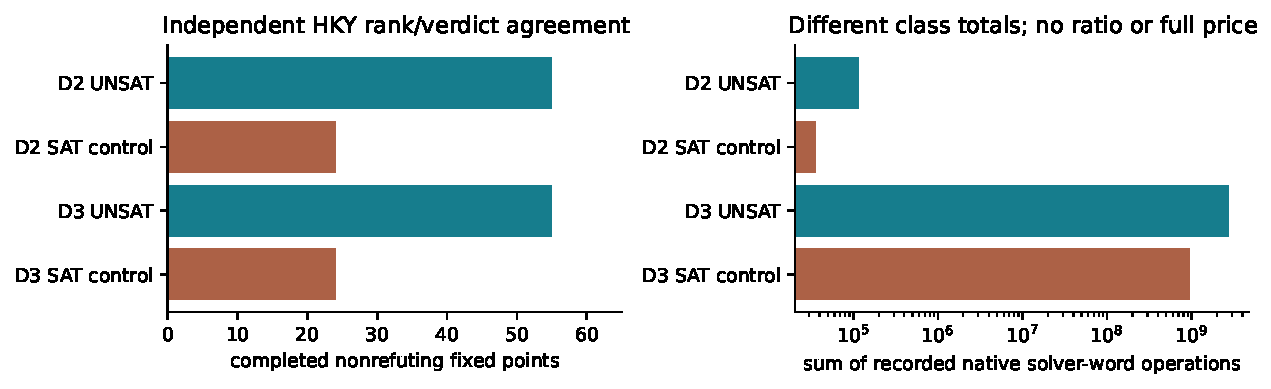
\includegraphics[width=\linewidth]{qualified-closure-coverage.pdf}\end{center}
\begin{center}\small\begin{tabular}{rlrrrr}\toprule
D & Class & Attempts & Nonrefuting & HKY checked & Solver words\\\midrule
2 & UNSAT & 55 & 55 & 55 & 113,834 \\
2 & SAT & 24 & 24 & 24 & 35,937 \\
3 & UNSAT & 55 & 55 & 55 & 2,719,392,090 \\
3 & SAT & 24 & 24 & 24 & 937,051,082 \\
\bottomrule\end{tabular}\end{center}
Every negative is finite-chain UNSAT and actual-subgroup UNSAT, has at least
two base points, is not a direct base hit, and is distinct in its file.
Every positive has both counts positive. The b-aware solver requires an
explicit SAT-control flag, and rejects any positive-control refutation.
Exact library and u128 polynomial equation builders agree before HKY replay.
The HKY engine uses independent monomial indexing, rounds and elimination;
its verdict/rank audit does not independently recount the producer's costs.

Producer source 35d265fc3, frozen binary SHA prefix 0b6c79f5a5df. Replay
source b98122f0b. Each process: one Rayon thread, column cap 40,000,
2-GiB address-space and 180-second cap. HKY_CHUNK=1024 for replay. Shared
AMD EPYC 9V74 Linux x86-64 host, L0. Diagnostic wall seconds are unqualified.

\textbf{Limits.} Nonrefuting closure does not prove SAT and does not prove
a degree law. This additional panel does not execute degree four or determine
the global minimum number of guesses. It does not discharge the original
b=1 all-branch campaign or larger-host shards. Construction, splitting,
point verification and native physical prices remain absent; the solver-word
totals are finite-stage counts, not complete query or DLP costs.
No cross-family performance ratio is formed because their selected queries
and bases differ. Original failed/capped runs are preserved separately.

Protocols: QUALIFIED_CLOSURE_PROTOCOL.md and QUALIFIED_CLOSURE_REPLAY_PROTOCOL.md.
Native source of this table/graph:
\path{../../pipeline-receipts/qualified-closure-replay-20261025/summary.json}.
All process records remain in the two separate raw run trees. No additional
paid VM allocation or artifact-store upload is claimed.

\end{document}
